\documentclass[11pt,a4paper,roman]{moderncv}        % possible options include font size ('10pt', '11pt' and '12pt'), paper size ('a4paper', 'letterpaper', 'a5paper', 'legalpaper', 'executivepaper' and 'landscape') and font family ('sans' and 'roman')

% moderncv themes
\moderncvstyle{casual}                             % style options are 'casual' (default), 'classic', 'oldstyle' and 'banking'
\moderncvcolor{purple}
%\usepackage{librebaskerville}                  % color options 'blue' (default), 'orange', 'green', 'red', 'purple', 'grey' and 'black'
\renewcommand{\familydefault}{\rmdefault}         % to set the default font; use '\sfdefault' for the default sans serif font, '\rmdefault' for the default roman one, or any tex font name
\nopagenumbers{}                                  % uncomment to suppress automatic page numbering for CVs longer than one page

% character encoding
%\usepackage[utf8]{inputenc}                       % if you are not using xelatex ou lualatex, replace by the encoding you are using
%\usepackage{CJKutf8}                              % if you need to use CJK to typeset your resume in Chinese, Japanese or Korean
\usepackage{graphicx}
% adjust the page margins
\usepackage[scale=0.75]{geometry}
%\setlength{\hintscolumnwidth}{3cm}                % if you want to change the width of the column with the dates
%\setlength{\makecvtitlenamewidth}{10cm}           % for the 'classic' style, if you want to force the width allocated to your name and avoid line breaks. be careful though, the length is normally calculated to avoid any overlap with your personal info; use this at your own typographical risks...

% personal data
\name{Sourav}{Basu}
\title{Curriculam Vit\ae{} -- "Courses of life"}                               % optional, remove / comment the line if not wanted
\address{Asansol}{}{India}% optional, remove / comment the line if not wanted; the "postcode city" and "country" arguments can be omitted or provided empty
\phone[mobile]{+91~9674085848}                   % optional, remove / comment the line if not wanted; the optional "type" of the phone can be "mobile" (default), "fixed" or "fax"
%\phone[fixed]{+2~(345)~678~901}
%\phone[fax]{+3~(456)~789~012}
\email{souravbasu17@gmail.com}                               % optional, remove / comment the line if not wanted
\homepage{souravbasu.com}                         % optional, remove / comment the line if not wanted
\social[linkedin][www.linkedin.com/souravbasu17]{Sourav Basu}                        % optional, remove / comment the line if not wanted
\social[github]{rmad17}                              % optional, remove / comment the line if not wanted
\social[twitter]{rmad1717}                             % optional, remove / comment the line if not wanted

%\extrainfo{additional information}                 % optional, remove / comment the line if not wanted
\photo[64pt][0.5pt]{picture}                       % optional, remove / comment the line if not wanted; '64pt' is the height the picture must be resized to, 0.4pt is the thickness of the frame around it (put it to 0pt for no frame) and 'picture' is the name of the picture file
\quote{passion, innovation and perfection!}                                 % optional, remove / comment the line if not wanted

% to show numerical labels in the bibliography (default is to show no labels); only useful if you make citations in your resume
%\makeatletter
%\renewcommand*{\bibliographyitemlabel}{\@biblabel{\arabic{enumiv}}}
%\makeatother
%\renewcommand*{\bibliographyitemlabel}{[\arabic{enumiv}]}% CONSIDER REPLACING THE ABOVE BY THIS

% bibliography with mutiple entries
%\usepackage{multibib}
%\newcites{book,misc}{{Books},{Others}}
%----------------------------------------------------------------------------------
%            content
%----------------------------------------------------------------------------------

\begin{document}

%\begin{CJK*}{UTF8}{gbsn}                          % to typeset your resume in Chinese using CJK
%-----       resume       ---------------------------------------------------------
\makecvtitle

\section{Education}
%\cventry{year--year}{Degree}{Institution}{City}{\textit{Grade}}{Description}  % arguments 3 to 6 can be left empty
\cventry{2009--13}{Bachelor of Technology}{Budge Budge Institute of Technology}{Kolkata}{\textit{7.86}}{}


\section{Theoretical Strengths}
\cvitem{}{Data Structure}
\cvitem{}{Algorithms}
\cvitem{}{Operating Systems}
\cvitem{}{}

\section{I converse in:}
\cvitemwithcomment{
\includegraphics[scale=0.4]{java-logo}}{{Java}}{Fluent Fundamentals}
\cvitemwithcomment{
\includegraphics[scale=0.3]{python}}{{Python}}{Development Allies}
\cvitemwithcomment{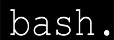
\includegraphics[scale=0.3]{bash}}{{Bash Scripting}}{Used as an utility}
\cvitemwithcomment{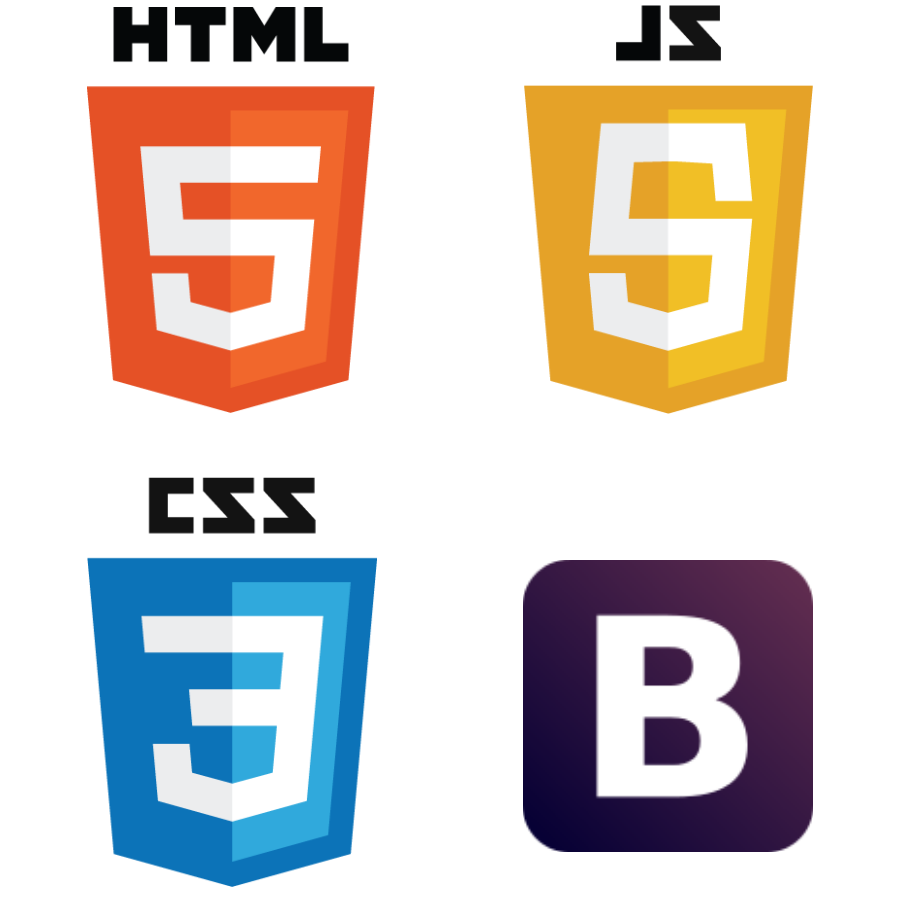
\includegraphics[scale=0.070]{HTML5}}{{HTML5, CSS, JS}}{Used sparingly}
\cvitem{}{}

\section{Platforms \& Frameworks:}
\cvitemwithcomment{
\includegraphics[scale=0.055]{android-logo}
}{{Android}}{Rich in experience}
\cvitemwithcomment{
\includegraphics[scale=0.023]{django-logo-negative}

\includegraphics[scale=0.085]{flask}}{{Django, FLask}}{Servers I use}
\cvitemwithcomment{
\includegraphics[scale=0.015]{hugo}}{{Hugo}}{Clay for my site}
\cvitem{}{}


\section{Technological Proficiency}
\cvitem{Linux Distributions}{\emph{Red Hat, Debian, CentOS, Ubuntu, Fedora and few others}}
\cvitem{Database}{\emph{Oracle, MySQL, PostgresSQL, SQLite, MongoDB}}
\cvitem{Others}{\emph{Git}}
\cvitem{}{}

%\cvitemwithcomment{}{}{ worked with}
%\cvitem{}{\emph{}}
%\cvdoubleitem{}{XXX, YYY, ZZZ}{category 5}{XXX, YYY, ZZZ}
%\cvdoubleitem{}{XXX, YYY, ZZZ}{category 6}{XXX, YYY, ZZZ}

\section{Open Source Contributions}
\cvitemwithcomment {Contributed}{Patch to DuckDuckGo search engine} {though unsuccesfully}
\cvitemwithcomment{Created}{Python Script to get Bitcoin values and notify me}{}
\cvitemwithcomment{Created}{Flask app to return random Wikipedia articles}{Added an android app as a client}
\cvitemwithcomment{Volunteered}{Fedora Project}{learnt about packaging maintainence}



\section{Experience}
%\subsection{Vocational}
\cventry{Jun - Dec, 2015}{Backend Engineer}{Appknox}{Bangalore}{}{Developed and maintained Django backend \newline{}}

\cventry{Apr 2014 - May 2015}{Associate Software Engineer}{LivQuik}{Mumbai}{}{Lead developer of the Quikwallet Android app\newline{}}

% Detailed achievements:%
% \begin{itemize}%
% \item Achievement 1;
% \item Achievement 2, with sub-achievements:
%  \begin{itemize}%
%  \item Sub-achievement (a);
% \item Sub-achievement (b), with sub-sub-achievements (don't do this!);
%    \begin{itemize}
%    \item Sub-sub-achievement i;
%    \item Sub-sub-achievement ii;
%    \item Sub-sub-achievement iii;
%    \end{itemize}
%  \item Sub-achievement (c);
%  \end{itemize}
% \item Achievement 3.
% \end{itemize}}
% \cventry{year--year}{Job title}{Employer}{City}{}{Description line 1\newline{}Description line 2}
%\subsection{Miscellaneous}
%\cventry{year--year}{Job title}{Employer}{City}{}{Description}





\section{Interests}
\cvlistitem{Watching Football, Tennis and Cricket.}
\cvlistitem{Learning new things, quizzing.}
\cvlistitem{UI/UX concepts}
\cvitem{}{}


%\section{FAQs}

\section{Why do I want to work for you?}
\cvlistitem{The scope of learning}
\cvlistitem{Chance to work with inquisitive and talented people}
%\cvlistitem{}
\cvitem{}{}

\section{Why should you hire me?}
\cvlistitem{My passion and creativity for innovation sets me aside from others. Like learning latex to create this CV.}
\cvlistitem{I am not the exceptional Django developer or Javascript magician. Neither am I the CentOS sys admin. On the contrarary I bring to your table a few good bit of everything. I bring to you versatility.}
\cvlistitem{Listening. I belive it to be a great tool for teamwork as to understand your team you have to \emph{listen}.}
\cvitem{}{}

% Publications from a BibTeX file without multibib
%  for numerical labels: \renewcommand{\bibliographyitemlabel}{\@biblabel{\arabic{enumiv}}}% CONSIDER MERGING WITH PREAMBLE PART
%  to redefine the heading string ("Publications"): \renewcommand{\refname}{Articles}
%\nocite{*}
%\bibliographystyle{plain}
%\bibliography{publications}                        % 'publications' is the name of a BibTeX file

% Publications from a BibTeX file using the multibib package
%\section{Publications}
%\nocitebook{book1,book2}
%\bibliographystylebook{plain}
%\bibliographybook{publications}                   % 'publications' is the name of a BibTeX file
%\nocitemisc{misc1,misc2,misc3}
%\bibliographystylemisc{plain}
%\bibliographymisc{publications}                   % 'publications' is the name of a BibTeX file

\clearpage


\end{document}
